\documentclass[UTF8,a4paper]{paper}
\usepackage{ctex}
\usepackage[utf8]{inputenc}
\usepackage{amsmath}
\usepackage{pdfpages}
\usepackage{graphicx}
\usepackage{wrapfig}
\usepackage{listings}
\usepackage{multicol}
\usepackage{float}
% Style definition file generated by highlight 3.6, http://www.andre-simon.de/ 

% Highlighting theme: Vim Editor 

\newcommand{\hlstd}[1]{\textcolor[rgb]{0,0,0}{#1}}
\newcommand{\hlnum}[1]{\textcolor[rgb]{1,0,0}{#1}}
\newcommand{\hlesc}[1]{\textcolor[rgb]{1,0.13,1}{#1}}
\newcommand{\hlstr}[1]{\textcolor[rgb]{1,0,0}{#1}}
\newcommand{\hlpps}[1]{\textcolor[rgb]{1,0,0}{#1}}
\newcommand{\hlslc}[1]{\textcolor[rgb]{0,0,1}{#1}}
\newcommand{\hlcom}[1]{\textcolor[rgb]{0,0,1}{#1}}
\newcommand{\hlppc}[1]{\textcolor[rgb]{1,0.13,1}{#1}}
\newcommand{\hlopt}[1]{\textcolor[rgb]{0,0,0}{#1}}
\newcommand{\hllin}[1]{\textcolor[rgb]{0,0,1}{#1}}
\newcommand{\hlkwa}[1]{\textcolor[rgb]{0.7,0.41,0.09}{#1}}
\newcommand{\hlkwb}[1]{\textcolor[rgb]{0,1,0}{#1}}
\newcommand{\hlkwc}[1]{\textcolor[rgb]{0.7,0.41,0.09}{#1}}
\newcommand{\hlkwd}[1]{\textcolor[rgb]{0,0,0}{#1}}
\definecolor{bgcolor}{rgb}{1,1,1}


\newcommand{\tabincell}[2]{\begin{tabular}{@{}#1@{}}#2\end{tabular}}
\title{实验五\ \ 综合设计电路实验}
\author{张蔚桐\ 2015011493\ 自55}
\begin {document}
\maketitle
\section{仿真和预习}
实验要求设计数字电压表,显示输入正弦波电压的峰值。因此考虑将电路分割为如下几个部分进行设计
\subsection{峰值提取部分}
这部分输入将输入的正弦波电压转换为尽可能稳定的输出电压,输出电压的值为输入正弦波的峰峰值。

具体的电路如图\ref{PP}所示,这是两个对称峰值检测电路分别检测电路的上峰值和下谷值。

其中,上半侧电路检测峰值,U1A为一个输入阻抗变换和U1B,二极管同时构成精密二极管,串接电容C6接地,完成正峰值检测。C6并联R10完成放电过程,方便动态检测电路。在U1B输出正向峰值。

下半部电路输出谷值,这里就不加赘述了。

输出之后进行R4C2的一个简单的一节低通滤波虑去前面C6放电出现的不稳定震荡,这方面R5C3,R8C4组成的简答低通滤波均完成此项内容,且效果稳定。

之后,U2A运放完成减法操作,检出峰峰值,之后滤波后阻抗变换跟随输出,稳定这个模块内部的工作,输出稳定电压。

经过仿真可以得到输出的电压准确度,稳定性均较好。

相对于娶她设计,这个电路能够应对多种波形输入,并且尤其适合中高频信号的输入。对于极低频信号,可能因为峰值检测电容放电的影响出现明显的纹波影响电路稳定性。

\begin{figure}\centering
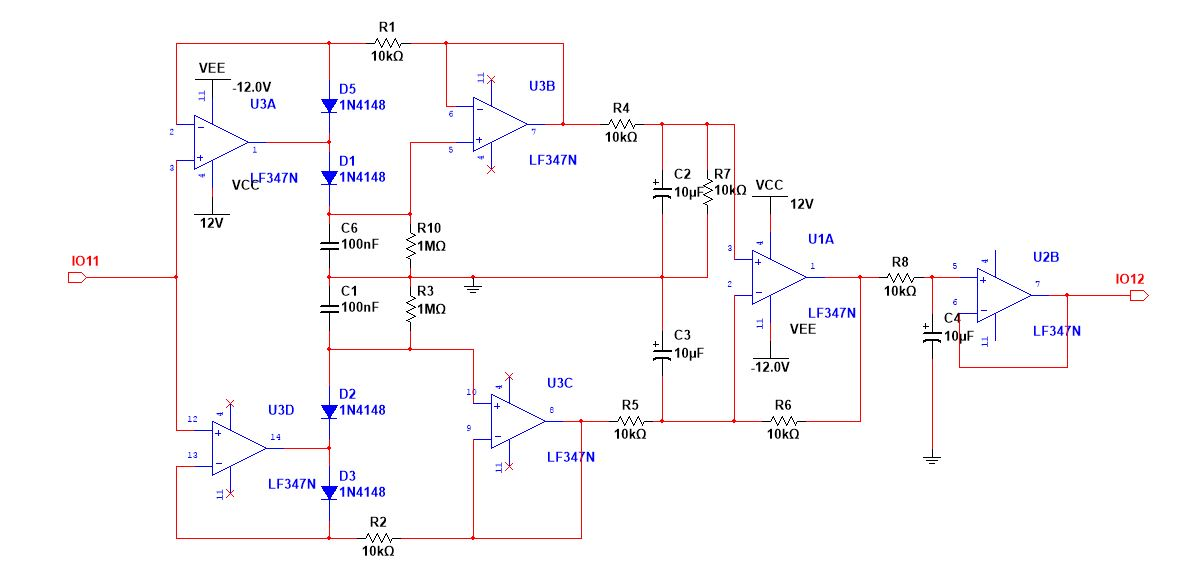
\includegraphics[width=\textwidth]{PP.jpg}
\caption{峰值提取电路}\label{PP}
\end{figure}
\subsection{电压转换部分}
这部分输入一个稳定的正电压,输出一个频率稳定的方波,具体的电路如图\ref{VF}所示
\begin{figure}[b]
\centering
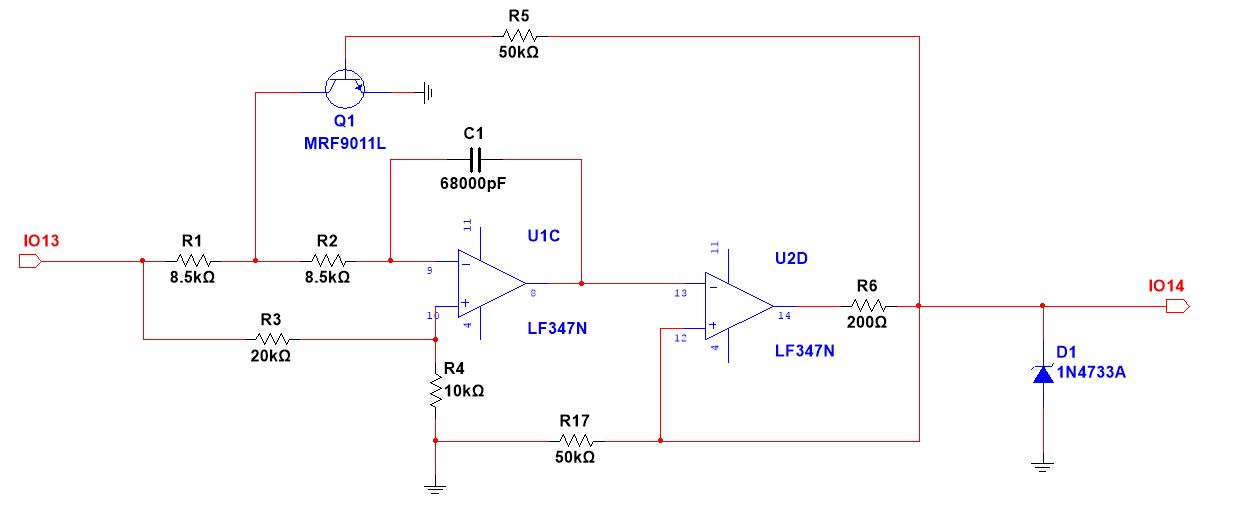
\includegraphics[width=\textwidth]{VF.jpg}
\caption{压频转换电路}
\label{VF}
\end{figure}

这个电路参考了模拟电子技术基础书上的压频转换电路的设计,具体原理略去。经过简单计算可以得到,电路在输入电压的控制下可以约为输出$50U_I\mathrm{Hz/V}$频率的方波,经过稳压之后输出共后级电路处理。

电路涉及的电阻较多,因此受到电阻型号和相对误差的影响,电路的具体的参数(如选择的电阻电容)选择在电路搭建的过程中也需要进一步的选取,这里的仿真就先略去。
\clearpage
\subsection{FPGA部分}
\begin {wrapfigure}{r}{0pt}
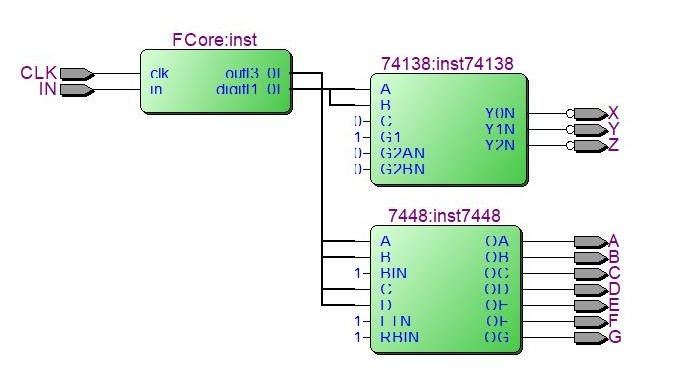
\includegraphics [width=60mm]{Block.jpg}
\caption{频率计数电路布置}
\label{DA}
\end {wrapfigure}
这部分要求将模拟电路输出的方波信号计数,得到最后要求显示的频率,为数字电路部分,电路模块图如图\ref{DA}所示。其中FCore模块是核心模块,负责在FPGA上的50MHz时钟下输出输入波形in的频率并在数码管中扫描显示。选通端由74138确定,数码管由7448驱动。

FCore模块的具体实现由Verilog代码给出。模块首先将输入时钟分频为1Hz,并在1Hz时钟上升沿设置输出记号。在输入in的每个上升沿,模块进行十进制计数。如果此时发现设置了输出记号,则清除此记号之后将当前值输出显示清零。

FCore也同时满足了一些诸如扫描数码管的功能,具体见下面的代码

\noindent
\ttfamily
\hlstd{}\hllin{01\ }\hlkwa{module\ }\hlstd{}\hlkwd{FCore\ }\hlstd{}\hlopt{(}\hlstd{clk}\hlopt{,}\hlstd{in}\hlopt{,}\hlstd{out}\hlopt{,}\hlstd{digit}\hlopt{);}\\
\hllin{02\ }\hlstd{}\hlkwa{input\ }\hlstd{clk}\hlopt{;}\\
\hllin{03\ }\hlstd{}\hlkwa{input\ }\hlstd{in}\hlopt{;}\\
\hllin{04\ }\hlstd{}\hlkwa{output\ }\hlstd{}\hlopt{{[}}\hlstd{}\hlnum{1}\hlstd{}\hlopt{:}\hlstd{}\hlnum{0}\hlstd{}\hlopt{{]}\ }\hlstd{digit}\hlopt{;}\\
\hllin{05\ }\hlstd{}\hlkwa{output\ }\hlstd{}\hlopt{{[}}\hlstd{}\hlnum{3}\hlstd{}\hlopt{:}\hlstd{}\hlnum{0}\hlstd{}\hlopt{{]}\ }\hlstd{out}\hlopt{;}\\
\hllin{06\ }\hlstd{}\hlkwa{reg\ }\hlstd{sec}\hlopt{;}\\
\hllin{07\ }\hlstd{}\hlkwa{reg\ }\hlstd{a\ }\hlopt{=\ }\hlstd{}\hlnum{0}\hlstd{}\hlopt{;}\\
\hllin{08\ }\hlstd{}\hlkwa{reg\ }\hlstd{b\ }\hlopt{=\ }\hlstd{}\hlnum{0}\hlstd{}\hlopt{;}\\
\hllin{09\ }\hlstd{}\hlkwa{reg\ }\hlstd{}\hlopt{{[}}\hlstd{}\hlnum{1}\hlstd{}\hlopt{:}\hlstd{}\hlnum{0}\hlstd{}\hlopt{{]}\ }\hlstd{digit\ }\hlopt{=\ }\hlstd{}\hlnum{2'b00}\hlstd{}\hlopt{;}\\
\hllin{10\ }\hlstd{}\hlkwa{reg\ }\hlstd{}\hlopt{{[}}\hlstd{}\hlnum{3}\hlstd{}\hlopt{:}\hlstd{}\hlnum{0}\hlstd{}\hlopt{{]}\ }\hlstd{out}\hlopt{;}\\
\hllin{11\ }\hlstd{}\hlkwa{reg\ }\hlstd{}\hlopt{{[}}\hlstd{}\hlnum{3}\hlstd{}\hlopt{:}\hlstd{}\hlnum{0}\hlstd{}\hlopt{{]}\ }\hlstd{num\ }\hlopt{{[}}\hlstd{}\hlnum{2}\hlstd{}\hlopt{:}\hlstd{}\hlnum{0}\hlstd{}\hlopt{{]};}\\
\hllin{12\ }\hlstd{}\hlkwa{reg\ }\hlstd{}\hlopt{{[}}\hlstd{}\hlnum{3}\hlstd{}\hlopt{:}\hlstd{}\hlnum{0}\hlstd{}\hlopt{{]}\ }\hlstd{\textunderscore num\ }\hlopt{{[}}\hlstd{}\hlnum{2}\hlstd{}\hlopt{:}\hlstd{}\hlnum{0}\hlstd{}\hlopt{{]};}\\
\hllin{13\ }\hlstd{}\hlkwa{reg\ }\hlstd{}\hlopt{{[}}\hlstd{}\hlnum{11}\hlstd{}\hlopt{:}\hlstd{}\hlnum{0}\hlstd{}\hlopt{{]}\ }\hlstd{div\ }\hlopt{=\ }\hlstd{}\hlnum{12'b1}\hlstd{}\hlopt{;}\\
\hllin{14\ }\hlstd{}\hlkwa{reg\ }\hlstd{}\hlopt{{[}}\hlstd{}\hlnum{27}\hlstd{}\hlopt{:}\hlstd{}\hlnum{0}\hlstd{}\hlopt{{]}\ }\hlstd{counter\ }\hlopt{=\ }\hlstd{}\hlnum{28'b0}\hlstd{}\hlopt{;}\\
\hllin{15\ }\hlstd{}\hlkwa{always\ }\hlstd{}\hlopt{@\ (}\hlstd{}\hlkwa{posedge\ }\hlstd{clk}\hlopt{)}\\
\hllin{16\ }\hlstd{}\hlkwa{begin}\\
\hllin{17\ }\hlstd{}\hlslc{//TODO:\ div\ the\ 50MHz\ clock\ to\ 1Hz}\\
\hllin{18\ }\hlstd{\ }\hlkwa{if}\hlstd{}\hlopt{(}\hlstd{counter\ }\hlopt{==\ }\hlstd{}\hlnum{28'd25000000}\hlstd{}\hlopt{)}\\
\hllin{19\ }\hlstd{\ }\hlkwa{begin}\\
\hllin{20\ }\hlstd{}\hlstd{\ \ }\hlstd{sec\ }\hlopt{$<$=\ $\sim$}\hlstd{sec}\hlopt{;}\\
\hllin{21\ }\hlstd{}\hlstd{\ \ }\hlstd{counter\ }\hlopt{=\ }\hlstd{}\hlnum{28'b1}\hlstd{}\hlopt{;}\\
\hllin{22\ }\hlstd{\ }\hlkwa{end}\\
\hllin{23\ }\hlstd{\ }\hlkwa{else\ }\\
\hllin{24\ }\hlstd{}\hlstd{\ \ }\hlstd{counter\ }\hlopt{$<$=\ }\hlstd{counter\ }\hlnum{+\ 1'b1}\hlstd{}\hlopt{;}\\
\hllin{25\ }\hlstd{}\hlstd{\ \ }\hlstd{\\
\hllin{26\ }\ }\hlslc{//TODO:\ div\ a\ sweeping\ signal}\\
\hllin{27\ }\hlstd{\ }\hlkwa{if}\hlstd{}\hlopt{(}\hlstd{div\ }\hlopt{==\ }\hlstd{}\hlnum{28'b0}\hlstd{}\hlopt{)}\\
\hllin{28\ }\hlstd{\ }\hlkwa{begin}\\
\hllin{29\ }\hlstd{}\hlstd{\ \ }\hlstd{div\ }\hlopt{$<$=\ }\hlstd{div\ }\hlnum{+\ 1'b1}\hlstd{}\hlopt{;}\\
\hllin{30\ }\hlstd{}\hlstd{\ \ }\hlstd{}\hlkwa{if}\hlstd{}\hlopt{(}\hlstd{digit\ }\hlopt{==\ }\hlstd{}\hlnum{2'b10}\hlstd{}\hlopt{)}\\
\hllin{31\ }\hlstd{}\hlstd{\ \ \ }\hlstd{digit\ }\hlopt{$<$=\ }\hlstd{}\hlnum{2'b00}\hlstd{}\hlopt{;}\\
\hllin{32\ }\hlstd{}\hlstd{\ \ }\hlstd{}\hlkwa{else}\\
\hllin{33\ }\hlstd{}\hlstd{\ \ \ }\hlstd{digit\ }\hlopt{$<$=\ }\hlstd{digit\ }\hlnum{+\ 1'b1}\hlstd{}\hlopt{;}\\
\hllin{34\ }\hlstd{\ }\hlkwa{end}\\
\hllin{35\ }\hlstd{\ }\hlkwa{else\ }\\
\hllin{36\ }\hlstd{}\hlstd{\ \ }\hlstd{div\ }\hlopt{$<$=\ }\hlstd{div\ }\hlnum{+\ 1'b1}\hlstd{}\hlopt{;}\\
\hllin{37\ }\hlstd{}\hlstd{\ \ }\hlstd{\\
\hllin{38\ }\ }\hlkwa{if}\hlstd{}\hlopt{(}\hlstd{div\ }\hlopt{==\ }\hlstd{}\hlnum{28'd10}\hlstd{}\hlopt{)}\\
\hllin{39\ }\hlstd{}\hlstd{\ \ }\hlstd{out\ }\hlopt{$<$=\ }\hlstd{num}\hlopt{{[}}\hlstd{digit}\hlopt{{]};}\\
\hllin{40\ }\hlstd{}\hlkwa{end}\\
\hllin{41\ }\hlstd{}\\
\hllin{42\ }\hlkwa{always\ }\hlstd{}\hlopt{@\ (}\hlstd{}\hlkwa{posedge\ }\hlstd{sec}\hlopt{)}\\
\hllin{43\ }\hlstd{}\hlkwa{begin}\\
\hllin{44\ }\hlstd{}\hlslc{//TODO:\ clear\ the\ output\ }\\
\hllin{45\ }\hlstd{a\ }\hlopt{$<$=\ $\sim$}\hlstd{b}\hlopt{;}\\
\hllin{46\ }\hlstd{}\hlkwa{end}\\
\hllin{47\ }\hlstd{}\\
\hllin{48\ }\hlkwa{always\ }\hlstd{}\hlopt{@\ (}\hlstd{}\hlkwa{posedge\ }\hlstd{in}\hlopt{)}\\
\hllin{49\ }\hlstd{}\hlkwa{begin}\\
\hllin{50\ }\hlstd{}\hlslc{//TODO:\ count}\\
\hllin{51\ }\hlstd{\ }\hlkwa{if}\hlstd{}\hlopt{(}\hlstd{a\ }\hlopt{==\ }\hlstd{b}\hlopt{)}\\
\hllin{52\ }\hlstd{\ }\hlkwa{begin}\\
\hllin{53\ }\hlstd{}\hlstd{\ \ }\hlstd{}\hlkwa{if}\hlstd{}\hlopt{(}\hlstd{\textunderscore num}\hlopt{{[}}\hlstd{}\hlnum{0}\hlstd{}\hlopt{{]}\ $<$\ }\hlstd{}\hlnum{4'd9}\hlstd{}\hlopt{)}\\
\hllin{54\ }\hlstd{}\hlstd{\ \ \ }\hlstd{\textunderscore num}\hlopt{{[}}\hlstd{}\hlnum{0}\hlstd{}\hlopt{{]}\ $<$=\ }\hlstd{\textunderscore num}\hlopt{{[}}\hlstd{}\hlnum{0}\hlstd{}\hlopt{{]}\ }\hlstd{}\hlnum{+\ 4'b0001}\hlstd{}\hlopt{;}\\
\hllin{55\ }\hlstd{}\hlstd{\ \ }\hlstd{}\hlkwa{else}\\
\hllin{56\ }\hlstd{}\hlstd{\ \ }\hlstd{}\hlkwa{begin}\\
\hllin{57\ }\hlstd{}\hlstd{\ \ \ }\hlstd{}\hlkwa{if}\hlstd{}\hlopt{(}\hlstd{\textunderscore num}\hlopt{{[}}\hlstd{}\hlnum{1}\hlstd{}\hlopt{{]}\ $<$\ }\hlstd{}\hlnum{4'd9}\hlstd{}\hlopt{)}\\
\hllin{58\ }\hlstd{}\hlstd{\ \ \ }\hlstd{}\hlkwa{begin\ }\\
\hllin{59\ }\hlstd{}\hlstd{\ \ \ \ }\hlstd{\textunderscore num}\hlopt{{[}}\hlstd{}\hlnum{1}\hlstd{}\hlopt{{]}\ $<$=\ }\hlstd{\textunderscore num}\hlopt{{[}}\hlstd{}\hlnum{1}\hlstd{}\hlopt{{]}\ }\hlstd{}\hlnum{+\ 4'b0001}\hlstd{}\hlopt{;}\\
\hllin{60\ }\hlstd{}\hlstd{\ \ \ \ }\hlstd{\textunderscore num}\hlopt{{[}}\hlstd{}\hlnum{0}\hlstd{}\hlopt{{]}\ $<$=\ }\hlstd{}\hlnum{4'b0000}\hlstd{}\hlopt{;}\\
\hllin{61\ }\hlstd{}\hlstd{\ \ \ }\hlstd{}\hlkwa{end}\\
\hllin{62\ }\hlstd{}\hlstd{\ \ \ }\hlstd{}\hlkwa{else}\\
\hllin{63\ }\hlstd{}\hlstd{\ \ \ }\hlstd{}\hlkwa{begin}\\
\hllin{64\ }\hlstd{}\hlstd{\ \ \ \ }\hlstd{\textunderscore num}\hlopt{{[}}\hlstd{}\hlnum{0}\hlstd{}\hlopt{{]}\ $<$=\ }\hlstd{}\hlnum{4'b0000}\hlstd{}\hlopt{;}\\
\hllin{65\ }\hlstd{}\hlstd{\ \ \ \ }\hlstd{\textunderscore num}\hlopt{{[}}\hlstd{}\hlnum{1}\hlstd{}\hlopt{{]}\ $<$=\ }\hlstd{}\hlnum{4'b0000}\hlstd{}\hlopt{;}\\
\hllin{66\ }\hlstd{}\hlstd{\ \ \ \ }\hlstd{\textunderscore num}\hlopt{{[}}\hlstd{}\hlnum{2}\hlstd{}\hlopt{{]}\ $<$=\ }\hlstd{\textunderscore num}\hlopt{{[}}\hlstd{}\hlnum{2}\hlstd{}\hlopt{{]}\ }\hlstd{}\hlnum{+\ 4'b0001}\hlstd{}\hlopt{;}\\
\hllin{67\ }\hlstd{}\hlstd{\ \ \ }\hlstd{}\hlkwa{end}\\
\hllin{68\ }\hlstd{}\hlstd{\ \ }\hlstd{}\hlkwa{end}\\
\hllin{69\ }\hlstd{\ }\hlkwa{end}\\
\hllin{70\ }\hlstd{\ }\hlkwa{else}\\
\hllin{71\ }\hlstd{\ }\hlkwa{begin}\\
\hllin{72\ }\hlstd{}\hlstd{\ \ }\hlstd{b\ }\hlopt{$<$=\ }\hlstd{a}\hlopt{;}\\
\hllin{73\ }\hlstd{}\hlstd{\ \ }\hlstd{num}\hlopt{{[}}\hlstd{}\hlnum{0}\hlstd{}\hlopt{{]}\ $<$=\ }\hlstd{\textunderscore num}\hlopt{{[}}\hlstd{}\hlnum{0}\hlstd{}\hlopt{{]};}\\
\hllin{74\ }\hlstd{}\hlstd{\ \ }\hlstd{num}\hlopt{{[}}\hlstd{}\hlnum{1}\hlstd{}\hlopt{{]}\ $<$=\ }\hlstd{\textunderscore num}\hlopt{{[}}\hlstd{}\hlnum{1}\hlstd{}\hlopt{{]};}\\
\hllin{75\ }\hlstd{}\hlstd{\ \ }\hlstd{num}\hlopt{{[}}\hlstd{}\hlnum{2}\hlstd{}\hlopt{{]}\ $<$=\ }\hlstd{\textunderscore num}\hlopt{{[}}\hlstd{}\hlnum{2}\hlstd{}\hlopt{{]};}\\
\hllin{76\ }\hlstd{}\hlstd{\ \ }\hlstd{\textunderscore num}\hlopt{{[}}\hlstd{}\hlnum{0}\hlstd{}\hlopt{{]}\ $<$=\ }\hlstd{}\hlnum{4'b0001}\hlstd{}\hlopt{;}\\
\hllin{77\ }\hlstd{}\hlstd{\ \ }\hlstd{\textunderscore num}\hlopt{{[}}\hlstd{}\hlnum{1}\hlstd{}\hlopt{{]}\ $<$=\ }\hlstd{}\hlnum{4'b0000}\hlstd{}\hlopt{;}\\
\hllin{78\ }\hlstd{}\hlstd{\ \ }\hlstd{\textunderscore num}\hlopt{{[}}\hlstd{}\hlnum{2}\hlstd{}\hlopt{{]}\ $<$=\ }\hlstd{}\hlnum{4'b0000}\hlstd{}\hlopt{;}\\
\hllin{79\ }\hlstd{\ }\hlkwa{end}\\
\hllin{80\ }\hlstd{}\hlkwa{end}\\
\hllin{81\ }\hlstd{}\hlkwa{endmodule}\hlstd{}\\
\mbox{}
\normalfont
\normalsize

\end{document}